\documentclass{article}

% Environment setup

\usepackage[
    margin=.75in
]{geometry} %geometry (sets margin) and other useful packages 

\setlength{\parindent}{0em}
\setlength{\parskip}{.75em}

\usepackage{graphicx}
\usepackage{grffile}  % support extra dots in filenames
\usepackage{fancyref}
\usepackage[labelfont=bf]{caption}
\usepackage{subcaption}


\title{\textbf{CS 4641:} Unsupervised Learning and Dimensionality Reduction}
\author{Bradley Reardon}
\date{March 24, 2019}

\begin{document}
  \maketitle

  \section{Introduction}
    TODO

    TODO datasets section

  \section{Clustering}
    TODO

    \subsection{$k$-means Clustering}
      TODO

      Car data set did not do well, testing with a subset of the whole set (since the set covers all possible instances) results in much more meaningful clusters with better scores. However, still not great at clustering this data set. For comparison, we use n\_clusters=4 since that matches the number of classes in the data, and clustering performed best on a subset with this value. Training time 0.117s

      TODO figures, figure refs \Fref{fig:km-silhouette-car}

      \begin{figure}[htb]
      \centering
      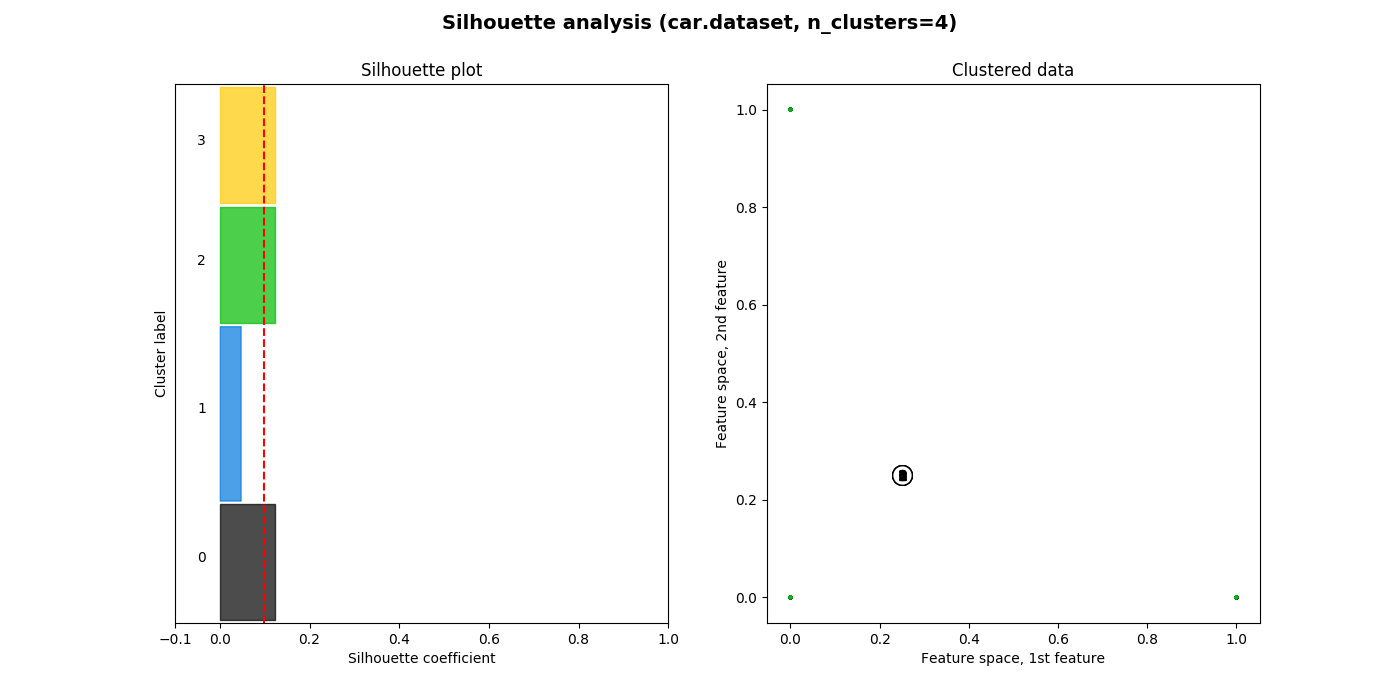
\includegraphics[width=\linewidth]{out/kmeans/car-4-clusters.png}
      \caption{Silhouette plot and clustered data visualization on two features for the car data set.}
      \label{fig:km-silhouette-car}
      \end{figure}

      Cancer data set performed much better, with a best-average silhouette score of 0.577 with n\_clusters=2, fit time 0.044s. Matches number of classes in the data set conveniently.

      TODO figures, figure refs \Fref{fig:km-silhouette-cancer}

      \begin{figure}[htb]
      \centering
      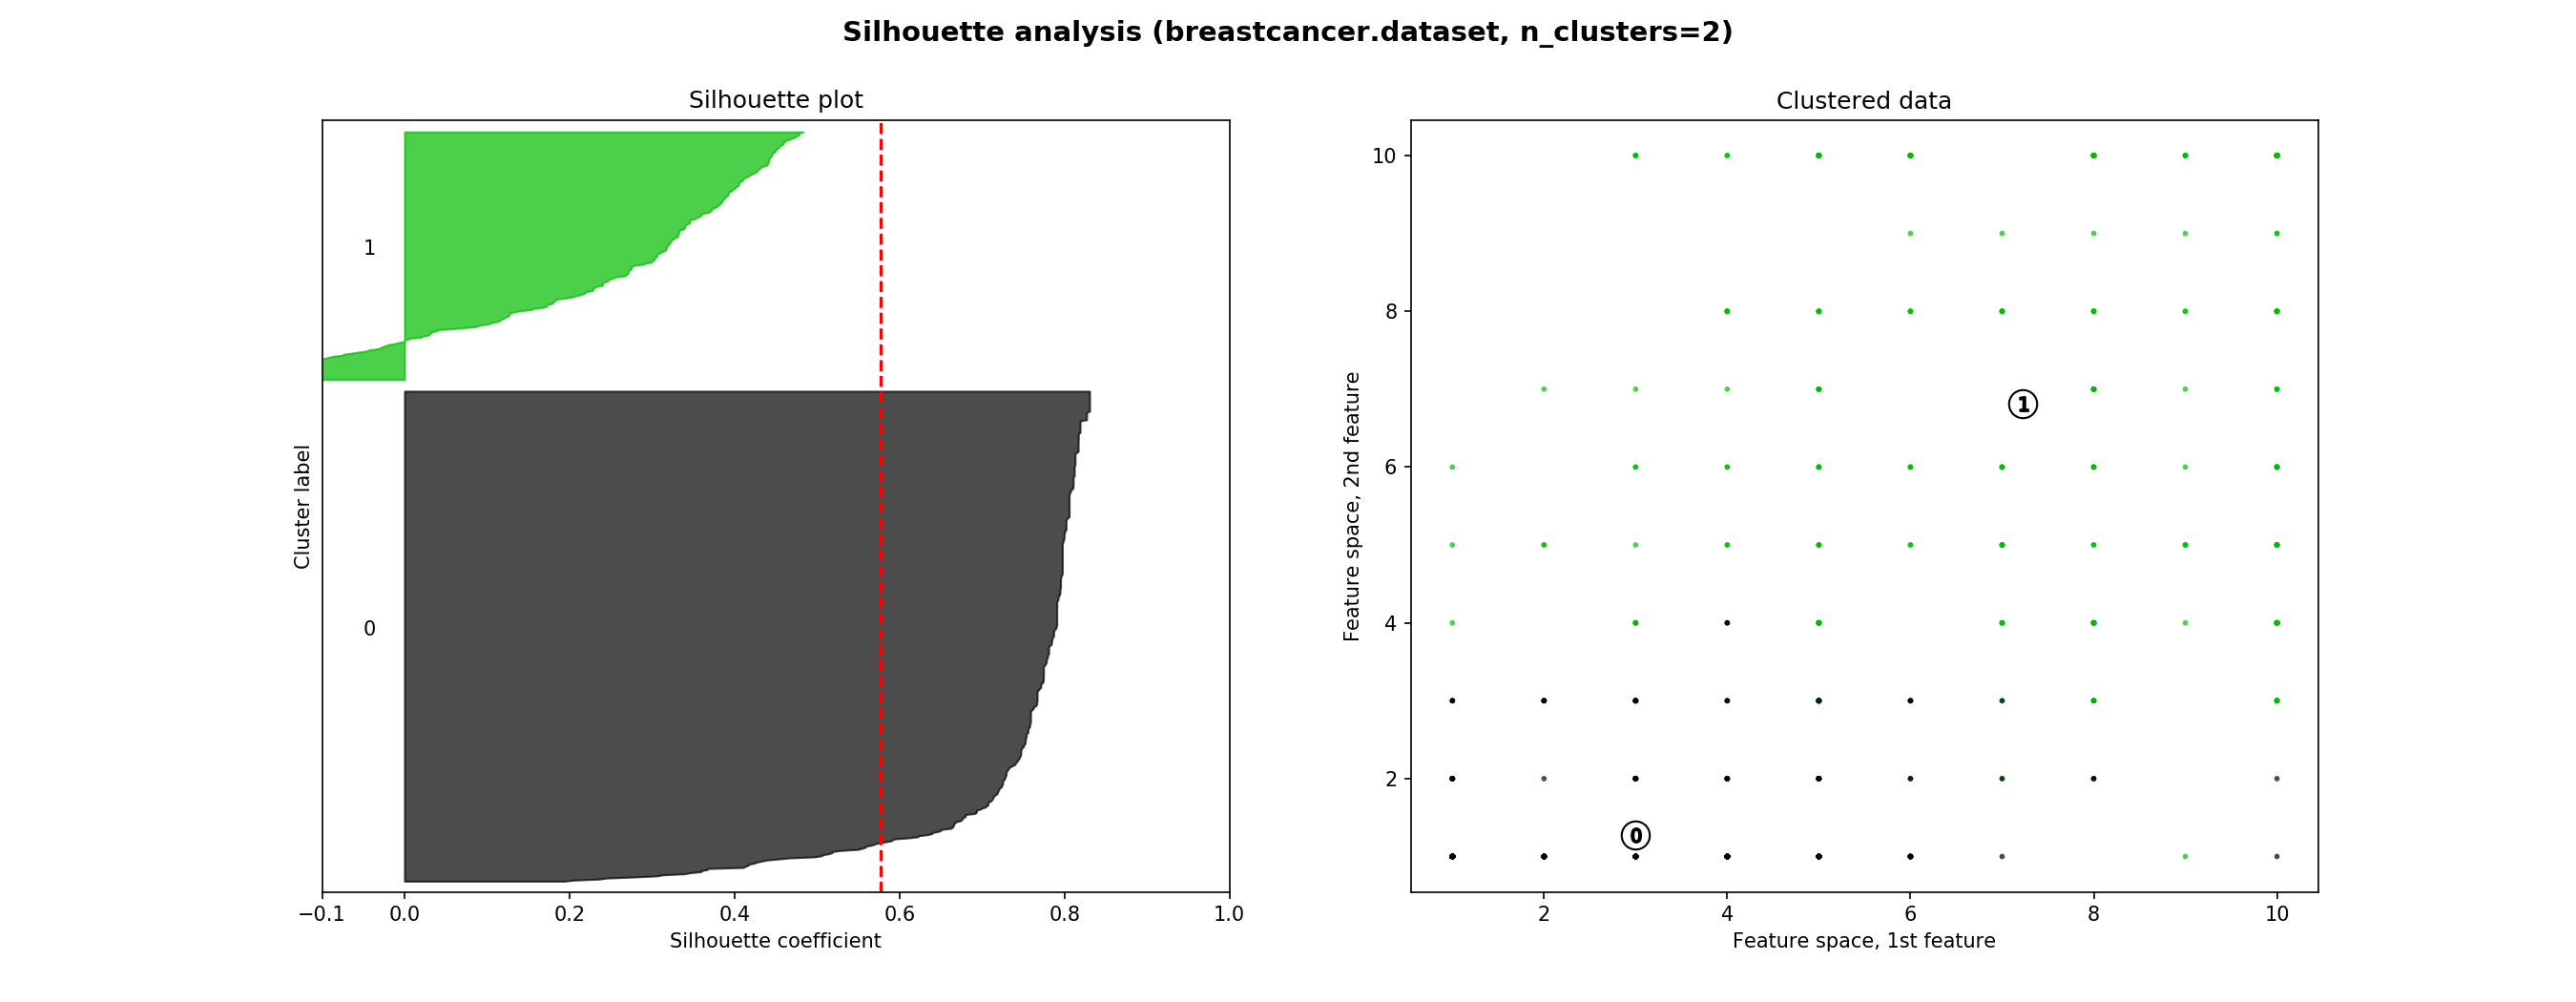
\includegraphics[width=\linewidth]{out/kmeans/cancer-2-clusters.png}
      \caption{Silhouette plot and clustered data visualization on two features for the cancer data set.}
      \label{fig:km-silhouette-cancer}
      \end{figure}

    \subsection{Expectation Maximization}
      TODO

    \subsection{Discussion}
      TODO talk about how the clusters aren't very well-defined in the charts, too many features.. try to reduce dimensionality in the next section to make that easier to see

  \section{Dimensionality Reduction}
    TODO

    \subsection{PCA}
      TODO

    \subsection{ICA}
      TODO

    \subsection{Randomized Projections}
      TODO

    \subsection{TODO pick feature selection algo}
      TODO

  \section{Conclusion}
    TODO

\end{document}